\documentclass[]{article}
\usepackage{lmodern}
\usepackage{amssymb,amsmath}
\usepackage{ifxetex,ifluatex}
\usepackage{fixltx2e} % provides \textsubscript
\ifnum 0\ifxetex 1\fi\ifluatex 1\fi=0 % if pdftex
  \usepackage[T1]{fontenc}
  \usepackage[utf8]{inputenc}
\else % if luatex or xelatex
  \ifxetex
    \usepackage{mathspec}
  \else
    \usepackage{fontspec}
  \fi
  \defaultfontfeatures{Ligatures=TeX,Scale=MatchLowercase}
\fi
% use upquote if available, for straight quotes in verbatim environments
\IfFileExists{upquote.sty}{\usepackage{upquote}}{}
% use microtype if available
\IfFileExists{microtype.sty}{%
\usepackage{microtype}
\UseMicrotypeSet[protrusion]{basicmath} % disable protrusion for tt fonts
}{}
\usepackage[margin=1in]{geometry}
\usepackage{hyperref}
\hypersetup{unicode=true,
            pdfborder={0 0 0},
            breaklinks=true}
\urlstyle{same}  % don't use monospace font for urls
\usepackage{longtable,booktabs}
\usepackage{graphicx,grffile}
\makeatletter
\def\maxwidth{\ifdim\Gin@nat@width>\linewidth\linewidth\else\Gin@nat@width\fi}
\def\maxheight{\ifdim\Gin@nat@height>\textheight\textheight\else\Gin@nat@height\fi}
\makeatother
% Scale images if necessary, so that they will not overflow the page
% margins by default, and it is still possible to overwrite the defaults
% using explicit options in \includegraphics[width, height, ...]{}
\setkeys{Gin}{width=\maxwidth,height=\maxheight,keepaspectratio}
\IfFileExists{parskip.sty}{%
\usepackage{parskip}
}{% else
\setlength{\parindent}{0pt}
\setlength{\parskip}{6pt plus 2pt minus 1pt}
}
\setlength{\emergencystretch}{3em}  % prevent overfull lines
\providecommand{\tightlist}{%
  \setlength{\itemsep}{0pt}\setlength{\parskip}{0pt}}
\setcounter{secnumdepth}{0}
% Redefines (sub)paragraphs to behave more like sections
\ifx\paragraph\undefined\else
\let\oldparagraph\paragraph
\renewcommand{\paragraph}[1]{\oldparagraph{#1}\mbox{}}
\fi
\ifx\subparagraph\undefined\else
\let\oldsubparagraph\subparagraph
\renewcommand{\subparagraph}[1]{\oldsubparagraph{#1}\mbox{}}
\fi

%%% Use protect on footnotes to avoid problems with footnotes in titles
\let\rmarkdownfootnote\footnote%
\def\footnote{\protect\rmarkdownfootnote}

%%% Change title format to be more compact
\usepackage{titling}

% Create subtitle command for use in maketitle
\newcommand{\subtitle}[1]{
  \posttitle{
    \begin{center}\large#1\end{center}
    }
}

\setlength{\droptitle}{-2em}

  \title{}
    \pretitle{\vspace{\droptitle}}
  \posttitle{}
    \author{}
    \preauthor{}\postauthor{}
    \date{}
    \predate{}\postdate{}
  

\begin{document}

\subsection{Introduction to the parameters that define a
sensor}\label{introduction-to-the-parameters-that-define-a-sensor}

We measure intensity at two wavelengths: \(I_{470}\) and \(I_{410}\) and
define the \(R = \frac{I_{410}}{I_{470}}\).

We calibrate our sensor such that we know the maximum and minimum
emission ratios, which we define as \(R_{max}\) and \(R_{min}\),
respectively.

We define a parameter \(\delta\) that describes a ratio between two
intensity wavelengths, one at a fully oxidized state and one at a fully
reduced state.
\(\delta_{\lambda} = \frac{I_{\lambda, oxidized}}{I_{\lambda, reduced}}\)

The dynamic range of the sensor as a whole is
\(\delta_R = \frac{I_{410, oxidized}}{I_{470, reduced}}\). The
\(\delta\) of the sensor at just one wavelength represents the
allocation of the sensor's total dynamic range in each wavelength. In
other words, \(\delta_R = \frac{\delta_{410}}{\delta_{470}}\). We will
use the allocation in one channel, \(\delta_{470}\) in future
calculations. In previous literature, \(\delta_{470}\) was referred to
as the `instrument factor', but it is characteristic of the sensor and
not any measuring instrument.

The maximum emission \(R_{max}\) and the minimum emission \(R_{min}\),
and therefore any measured value \(R\), will vary depending on the
parameters of the microscope with which they were measured. To
standardize these calculations to any microscope, we define a
standardized ratio \(R' = \frac{R}{R_{min}}\), in which \(R'_{min} = 1\)
and \(R'_{max} = \frac{R_{max}}{R_{min}}\). This parameter scaling can
apply to any of the calculations below without changing the underlying
arithmetic.

\subsection{Converting between measured ratio, fraction of sensors
oxidized, and redox
potential}\label{converting-between-measured-ratio-fraction-of-sensors-oxidized-and-redox-potential}

We can use the properties of the sensor to infer the fraction of sensor
molecules that are in an oxidized state \(OxD\) at any given \(R\).

\[ OxD = \frac{R-R_{min}}{R-R{min} + \delta_{470}(R_{max} - R)} \].

Values of \(OxD\) vary between \(0\), when \(R = R_{min}\), and \(1\),
when \(R = R_{max}\). When \(\delta_{470} = 1\), there is a linear
relationship between \(R\) and \(OxD\)
(\(OxD = \frac{R-R_{min}}{R-R{min} + 1 * (R_{max} - R)} = \frac{R-R_{min}}{R_{min} + R_{max}}\)).
At any \(|\delta_{470} - 1| > 0\), the relationship is nonlinear.

We can similarily convert R to a redox potential via the Nernst
potential. In terms of the fraction oxidized:

\[E = E^\circ - \frac{RT}{2F}ln(\frac{1-OxD}{OxD})\].

In terms of R, this simplifies to:

\[E = E^\circ - \frac{R_{gas}T}{2F}ln(\frac{\delta_{470}*(R_{max}-R)}{R-R_{min}})\]

Values of \(E\) vary between \(-\infty\) and \(+\infty\). When the
measured ratio is halfway between the minimum and maximum ratios
(\(R = \frac{R_{min} + R_{max}}{2})\)), the value of \(E\) reaches a
point that we call the adjusted midpoint potential \(E^\circ_{adj}\),
which we define as
\(E^\circ_{adj} = E^\circ - \frac{R_{gas}T}{2F}ln(\delta_{470)})\). In
other words, when \(\delta_{470} = 1\), the adjusted midpoint potential
is equal to the midpoint potential of the sensor
\(E^\circ_{adj} = E^\circ\). \(\delta_{470}\) values above 1 decrease
the adjusted midpoint potential, whereas values below 1 increase the
adjusted midpoint potential.

\begin{center}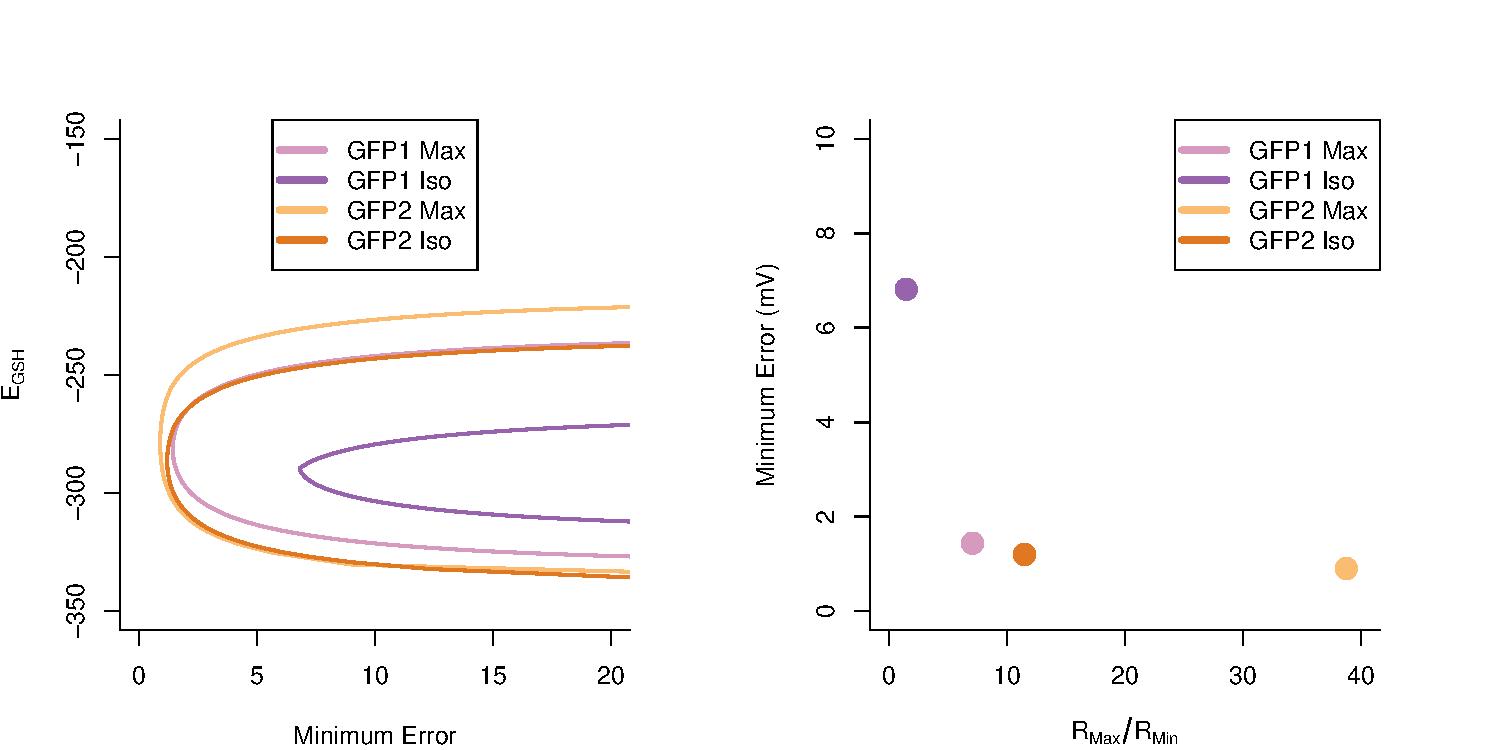
\includegraphics{Final_Main_files/figure-latex/unnamed-chunk-1-1} \end{center}

\textbf{Figure 1}. Measured ratio values of \(R\) can be converted to
the fraction oxidized \(OxD\) or the redox potential \(E\). This figure
is plotted based on a hypothetical sensor with
\(\{R_{min}, R_{max}, E^\circ\} = \{1, 5, -270 mV\}\). The parameter
\(\delta_{470}\) changes the linearity of the map to \(OxD\), whereas it
changes the adjusted midpoint potential of the map to \(E\)

\subsection{Sensitivity analysis}\label{sensitivity-analysis}

In a real-world experiment, there is likely to be some empirical error
in the measured value of R. The inferred values of OxD and E will incur
some level of error as a result of an error of R. The relative amount of
error in OxD or E as a result of errors in R may vary depending on where
in the range of \(R_{min}\) to \(R_{max}\) the real value of \(R\) lies.

The theoretical relative errors of values of E and OxD at any given
\(R\) are defined by the respective derivatives with respect to R of
each mapping:

The sensitivity of OxD is dependent on all of the sensor's parameters:
\[\frac{\partial OxD}{\partial R} = \frac{\delta_{470}(R_{max}-R_{min})}{(R(\delta_{470} - 1) - \delta_{470}R_{max} + R_{min})^2}\]

The sensitivity of E with respect to R is only dependent on \(R\),
\(R_{min}\), and \(R_{max}\):
\[\frac{\partial E}{\partial R} = \frac{-RT}{2F}*\frac{R_{max}-R_{min}}{(R-R_{min})(R-R_{max})}\]

\begin{center}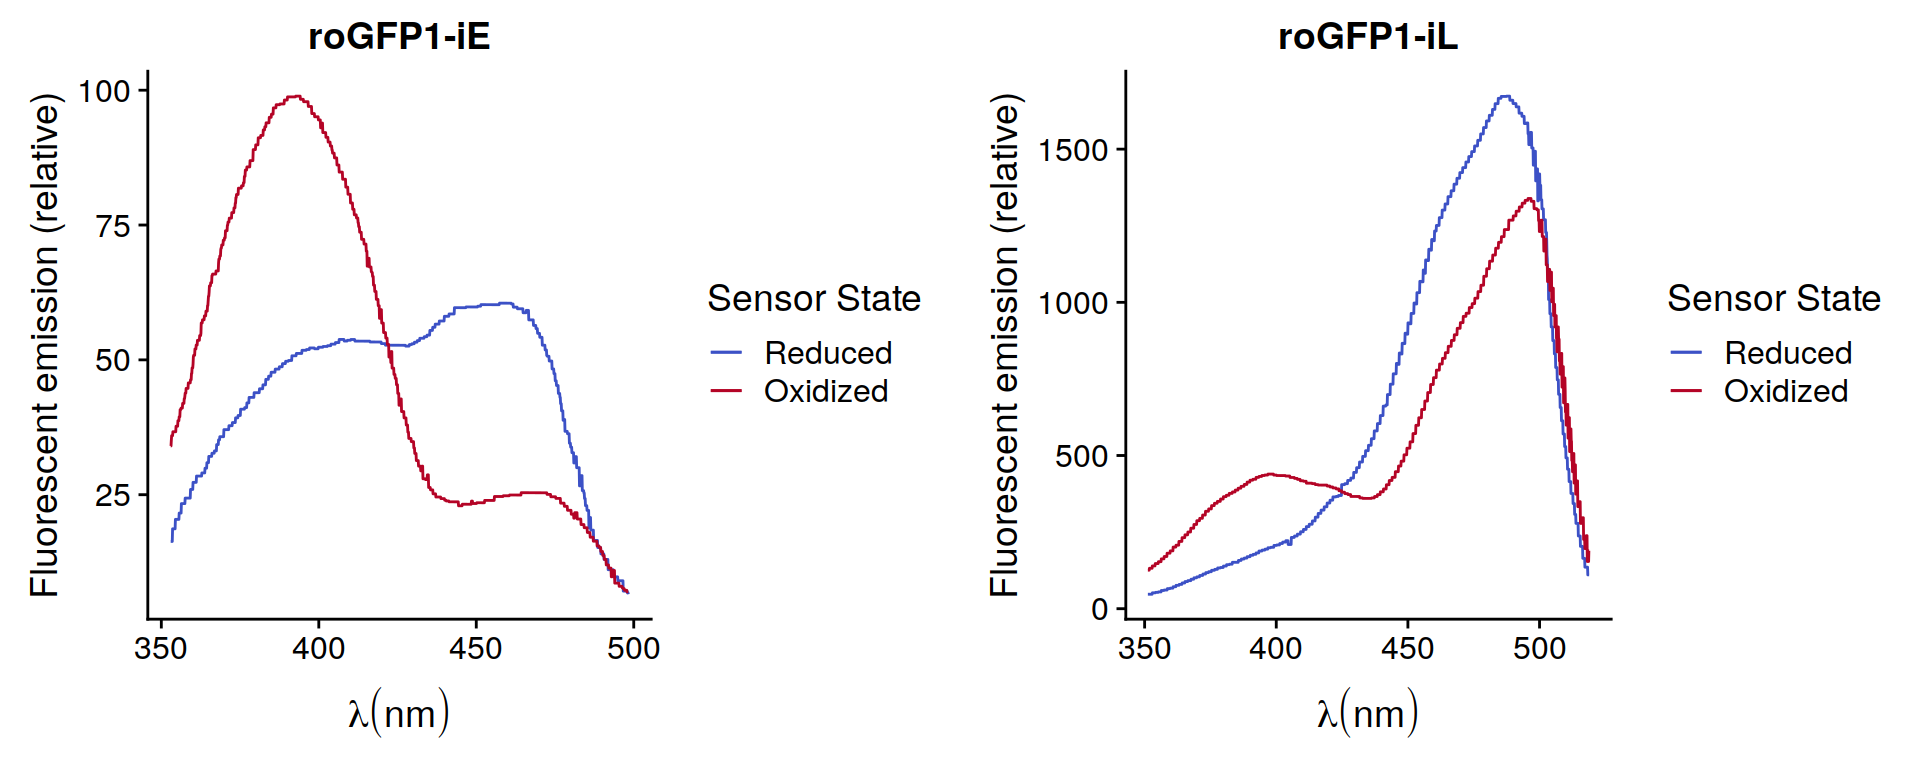
\includegraphics{Final_Main_files/figure-latex/unnamed-chunk-2-1} \end{center}

\textbf{Figure 2}. Mappings of \(R\) to \(OxD\) and \(E\) and their
respective derivatives. This figure is plotted based on a hypothetical
sensor with
\(\{R_{min}, R_{max}, \delta_{470}, E^\circ\} = \{1, 5, 0.2, -270 mV\}\).

For our purposes, we are most concerned with how errors in \(R\)
propagate to errors in \(E\). Or, more importantly, the errors in \(E\)
at different levels of real redox potential.

\begin{center}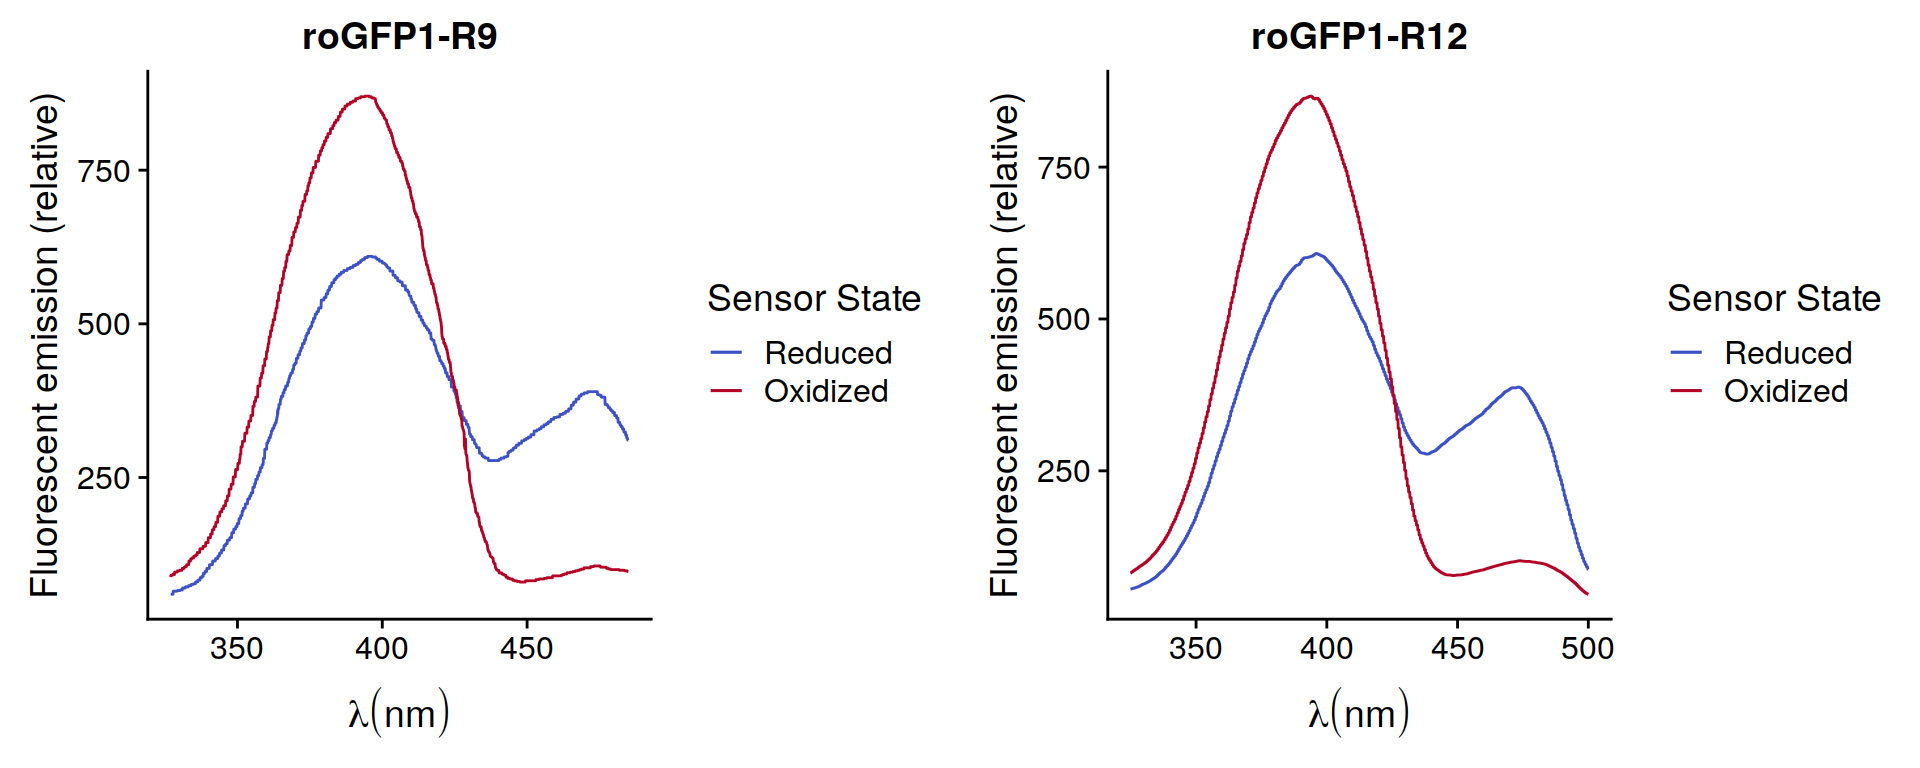
\includegraphics{Final_Main_files/figure-latex/unnamed-chunk-3-1} \end{center}

\textbf{Figure 3}. The discrepancy between actual redox potential and
recorded redox potential at a given measurement of R (left) or
corresponding E (right). This figure is plotted based on a hypothetical
sensor with
\(\{R_{min}, R_{max}, \delta_{470}, E^\circ\} = \{1, 5, 0.2, -270 mV\}\).

At a given level of error in \(R\),, there is a range of \(E\) values
that are defined at every level of error in \(E\)

\begin{center}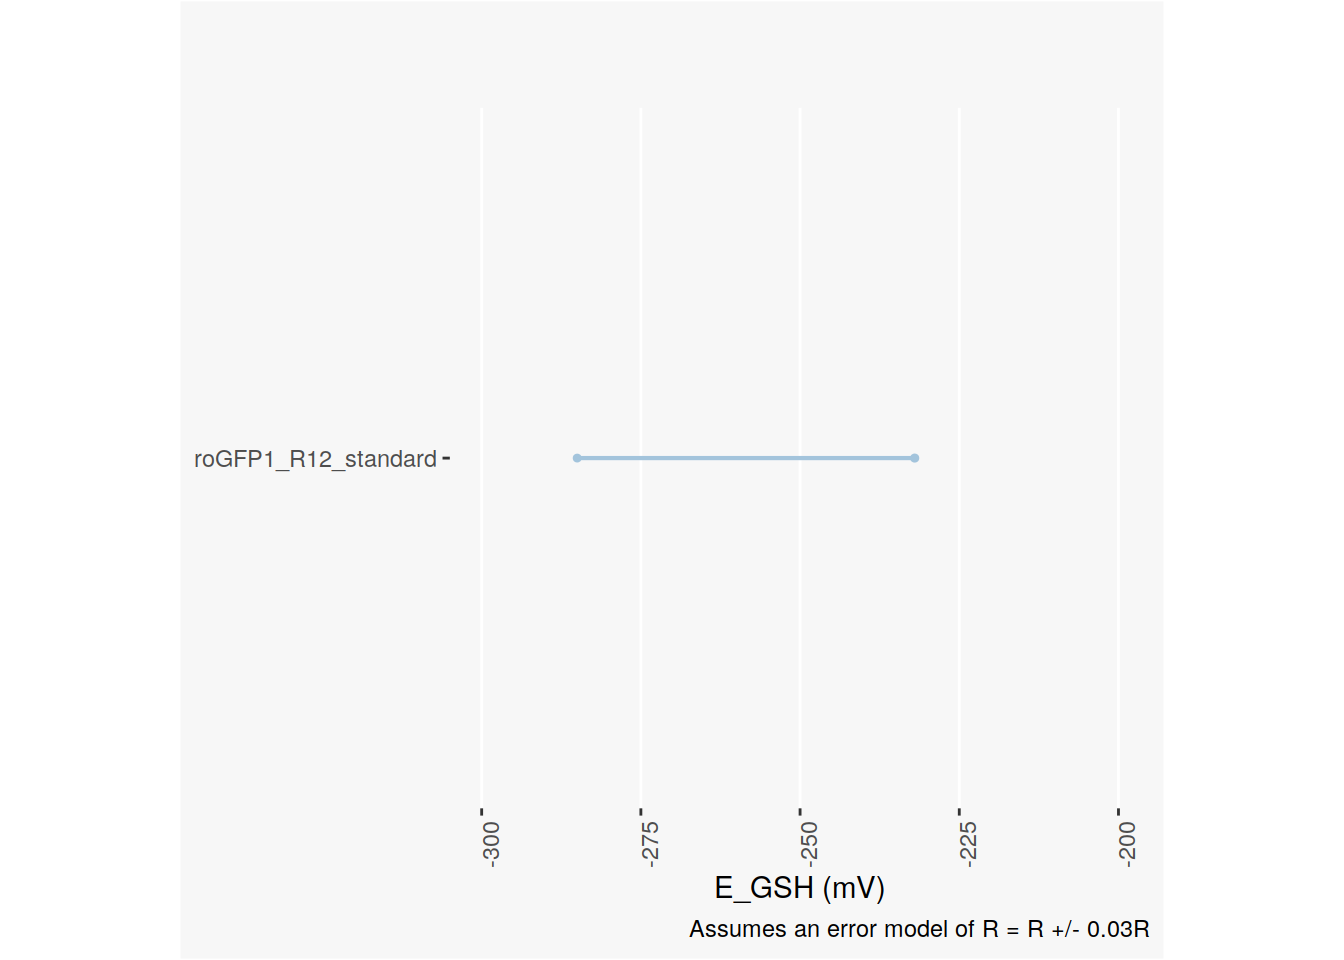
\includegraphics{Final_Main_files/figure-latex/unnamed-chunk-4-1} \end{center}

\textbf{Figure 4}. A phase diagram of minimum and maximum detectable
redox potentials, given an error in R of 5\%. This figure is plotted
based on a hypothetical sensor with
\(\{R_{min}, R_{max}, \delta_{470}, E^\circ\} = \{1, 5, 0.2, -270 mV\}\).

\subsection{Applying the sensitivity analysis to roGFP1 and
roGFP2}\label{applying-the-sensitivity-analysis-to-rogfp1-and-rogfp2}

roGFP1 and roGFP2 have different properties, based on their emission
spectra

\begin{center}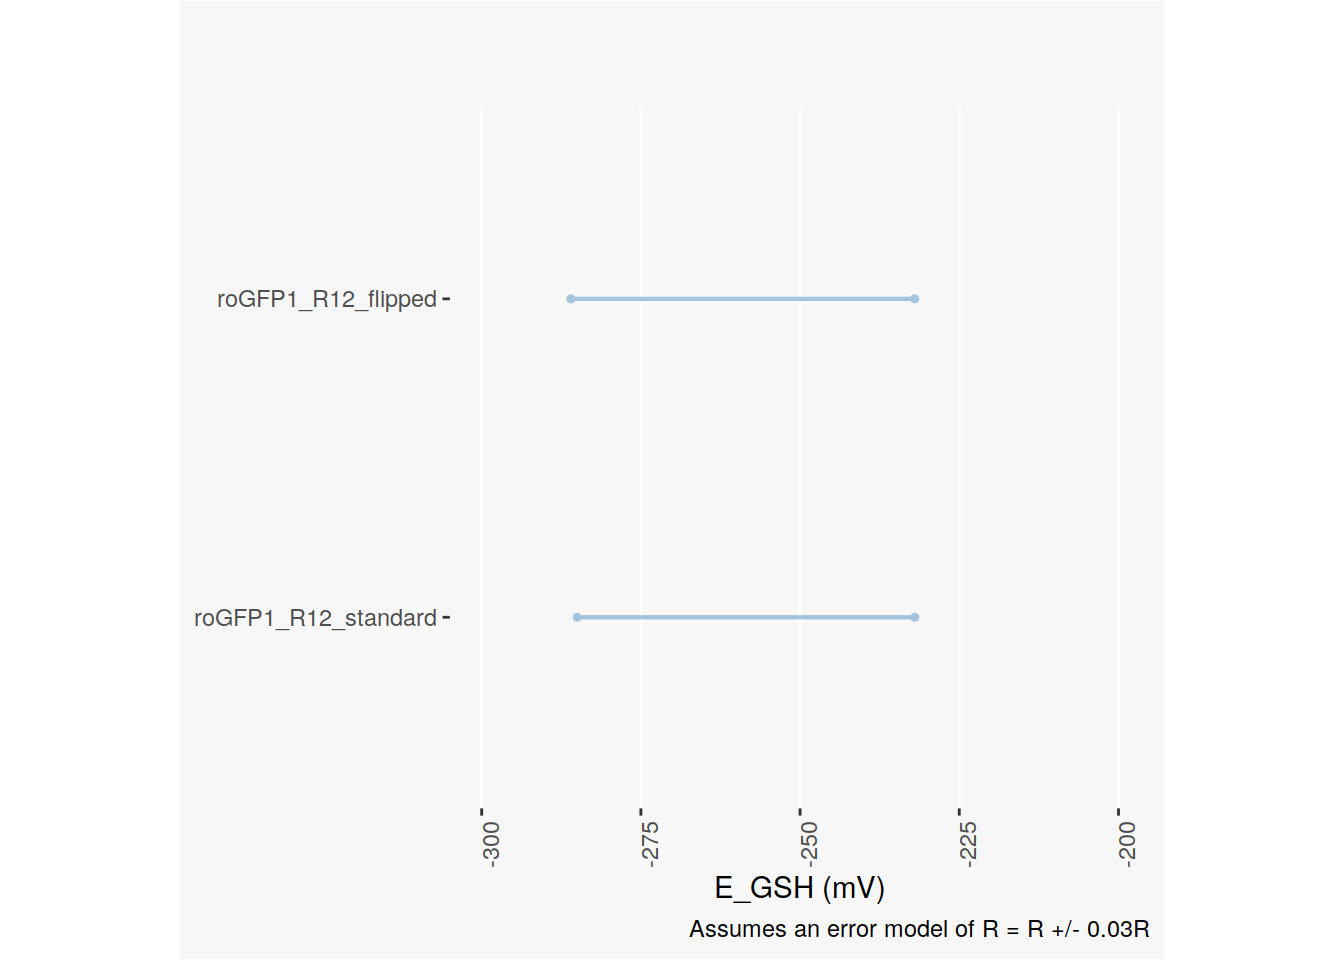
\includegraphics{Final_Main_files/figure-latex/unnamed-chunk-6-1} \end{center}

\begin{longtable}[]{@{}lll@{}}
\caption{Table 1: Characteristics of GFP1 and GFP2
sensors}\tabularnewline
\toprule
Name: & GFP1 & GFP2\tabularnewline
\midrule
\endfirsthead
\toprule
Name: & GFP1 & GFP2\tabularnewline
\midrule
\endhead
Rmax & 27.01 & 0.634\tabularnewline
Rmin & 4.098 & 0.094\tabularnewline
Delta & 0.250 & 0.481\tabularnewline
E0 & -288 & -272\tabularnewline
\bottomrule
\end{longtable}

\begin{center}\includegraphics{Final_Main_files/figure-latex/unnamed-chunk-8-1} \end{center}


\end{document}
